
\documentclass[a4paper,12pt]{report}
\usepackage{graphicx} % Per inserire immagini
\usepackage{fancyhdr} % Per gestire l'intestazione e il piè di pagina
\usepackage{geometry} % Per gestire i margini
\geometry{a4paper, margin=1in} % Margini della pagina
\usepackage{tocbibind} % Per includere l'indice e la bibliografia nell'indice
\usepackage{hyperref} % Per i collegamenti interni nell'indice
\usepackage{amsmath} % Pacchetto utile per formule matematiche
\usepackage{amssymb} % Per \mathbb
\usepackage{enumitem} % Pacchetto per personalizzare gli elenchi
\usepackage{listings}
%\usepackage{xcolor}
\usepackage{tabularx}
\usepackage[table,xcdraw]{xcolor}
%\usepackage{listings}
\usepackage{matlab-prettifier}
\usepackage{mathtools}
\usepackage[utf8]{inputenc}
\usepackage{listings} % Package for code formatting
\usepackage{xcolor}   % For defining colors for code highlighting
\usepackage{subcaption} % For subfigures

% Define code style for listings
\lstdefinestyle{codeStyle}{
    backgroundcolor=\color{lightgray!20},   
    basicstyle=\footnotesize\ttfamily,
    breaklines=true,  
    frame=single,
    numbers=left,
    numberstyle=\tiny\color{gray},
    keywordstyle=\color{blue},
    commentstyle=\color{green},
    stringstyle=\color{orange},
}

% Configurazione dell'intestazione (dopo l'indice)
\fancypagestyle{aftertoc}{%
    \fancyhf{} % Pulisce intestazione e piè di pagina
    \fancyhead[L]{
\includegraphics[width=0.05\textwidth]{IST_Logo.png}} % Aggiunge il logo a sinistra
    \fancyhead[R]{\textit{Optimization and Algorithms}} % Aggiunge il testo a destra
    \renewcommand{\headrulewidth}{0.4pt} % Linea sotto l'intestazione
}

\begin{document}

% Titolo principale
\begin{center}
    \textbf{\LARGE Instituto Superior Técnico, Universidade de Lisboa} \\[1cm]
    % Logo
    
\includegraphics[width=0.2\textwidth]{IST_Logo.png} \\[1cm]
    \textbf{\Large Master of Science in Electrical and Computer Engineering} \\[1cm]
    \textbf{\large A.Y. 2024/2025} \\[1cm]
    \textit{\Large Optimization and Algorithms Project} \\[1cm]
\end{center}

\vfill % Questo comando forza il contenuto a riempire verticalmente la pagina

% Informazioni sui professori
\noindent
\begin{tabular}{ll}
    {\large \bfseries Professores:} & {\large  Joao Xavier, Joao Sequeira, Hugo Pereira } 
\end{tabular}

\vfill % Aggiunge spazio verticale tra la sezione dei professori e quella del gruppo

% Informazioni sul gruppo
\noindent
\textbf{Group 1:} \\
\begin{itemize}
    \item Lino Di Lucia (ist1112859) - lino.dilucia@studentmail.unicas.it
    \item Pascal Seitter (ist1112432) - pascal.seitter@tum.de
    \item João Costa (ist199088) - joaoarcosta@tecnico.ulisboa.pt
    \item Matteo Talè (ist1113101) - matteo.tale@tecnico.ulisboa.pt
\end{itemize}

% Inserimento dell'indice
\renewcommand{\contentsname}{Index}
\tableofcontents

\newpage % Passa a una nuova pagina dopo l'indice

% Attivazione del nuovo stile di pagina (dopo l'indice)
\pagestyle{aftertoc}

\chapter{Aim of the project}
This project aims to solve some tasks assigned in class. For the analysis of the respective tasks, it was necessary to use MATLAB and the CVX tool (important in solving problems of a convex nature). The tasks are divided into theoretical tasks for which a graphical and/or analytical solution was presented and numerical tasks, for which the code will be shown in detail and the final result.

\section{Task 1: Examination of non convexity}

The goal of this task is to demonstrate that the function \( f_D \) defined as
\begin{equation} \label{eq:fd_full}
    \frac{1}{N} \sum_{n=1}^{N} 1_{R_-}(y_n C_{w_0, w}(x_n))
\end{equation}
is not convex. We will focus on a simple case where \( N = 1 \) and \( D = 1 \).

For the case where \( N = 1 \) and \( D = 1 \), this simplifies to:
\begin{equation} \label{eq:fd_simple}
    f_D =  1_{R_-}( y_1 C_{w_0,w}(x_1) )
\end{equation}


To illustrate the non-convexity of \( f_D \), we can analyze the graph of the function for specific values of \textit{y\(_1\)}, \textit{C}, and \textit{w(x\(_1\))}. The non-convexity becomes evident when the graph exhibits a shape that fails to meet the definition of convexity — specifically, when the line segment connecting any two points on the graph does not lie entirely above the graph.

Rather than substituting all the values of \textit{x\(_1\)}, \textit{y\(_1\)}, \textit{w\(_0\)}, and \textit{w\(_1\)} into the definition of a convex function, as discussed in class, it is far more practical to perform a straightforward plot of the function for the case under consideration. This visual approach allows for a clear identification of the non-convex behavior.

 \newpage

\begin{figure}[h]
        \centering
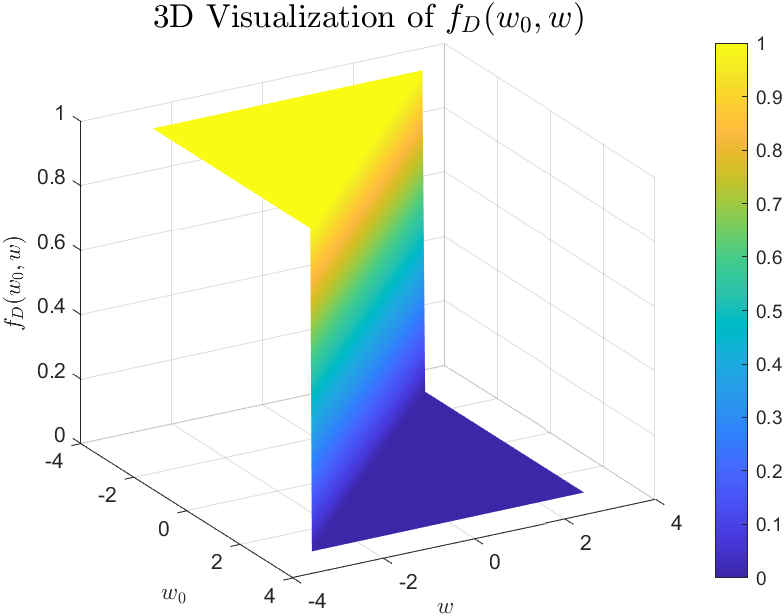
\includegraphics[width=1\linewidth]{task_1.png}
                \centering
    \caption{Graph illustrating the non-convexity of the function \( f_D \) for the case \( N = 1 \) and \( D = 1 \).}
    \label{fig:non_convexity}
\end{figure}

\textbf{Geometrical interpretation:} The graph above demonstrates that the function \( f_D \) is not convex, as evidenced by the fact that the line segment connecting two points on the curve does not lie entirely above the curve itself.In other words, if two points that are chosen on the graph, where one point has the function value 1 and the other point has the function value 0, and both points are connected with a straight line, it can be clearly seen that the graph does not lie completely below this straight line between those two points and thus violates the condition of convexity that from a geometrical point of view requires that the chord is above the graph .This confirms our assertion regarding the non-convexity of the function for the specified case.

\section{Task 2: Comparison of $\mathbf{1}_{\mathbb{R}_-}$ and Hinge Loss}

Our goal is to show that the function \( \mathbf{1}_{\mathbb{R}_-} \), defined as:
\begin{equation} \label{eq:indicator}
\mathbf{1}_{\mathbb{R}_-}(u) = \begin{cases}
1 & \text{if } u < 0, \\
0 & \text{if } u \geq 0,
\end{cases}
\end{equation}
is majorized by the hinge loss function \( h(u) = (1 - u)_+ \), where the hinge loss is defined as:
\begin{equation} \label{eq:hinge_loss}
h(u) = \max(0, 1 - u).
\end{equation}
In other words, we need to prove that $\mathbf{1}_{\mathbb{R}_-}(u) \leq h(u)$ for all $u \in \mathbb{R}$.

\subsection{Analytical Proof}

We define the following auxiliary function for positive values of \( u \), denoted by \( \mathbf{1}_{\mathbb{R}_+}(u) \):
\begin{equation} \label{eq:indicator_positive}
\mathbf{1}_{\mathbb{R}_+}(u) = \begin{cases}
1 & \text{if } u > 0, \\
0 & \text{otherwise}.
\end{cases}
\end{equation}

We have the relation:
\begin{equation} \label{eq:relation}
\mathbf{1}_{\mathbb{R}_-}(u) = \mathbf{1}_{\mathbb{R}_+}(-u).
\end{equation}

Analyzing the cases:

\begin{itemize}
    \item For $u < 0$: $\mathbf{1}_{\mathbb{R}_+}(-u) = 1$. Therefore, $h(u) = \max(0, 1 - u) = 1 - u \geq 1$ (since $u < 0$). Thus, $\mathbf{1}_{\mathbb{R}_-}(u) = 1 \leq h(u)$.
    \item For $u \geq 0$: $\mathbf{1}_{\mathbb{R}_+}(-u) = 0$, and $h(u) = \max(0, 1 - u) = 0$. Therefore, $\mathbf{1}_{\mathbb{R}_-}(u) = 0 \leq h(u)$.
\item we can conclude:
\[
\mathbf{1}_{\mathbb{R}_-}(u) = \mathbf{1}_{\mathbb{R}_+}(-u) \leq \max(0, 1 - u) = h(u) = (1 - u)_+
\]
This completes the analytical proof that $\mathbf{1}_{\mathbb{R}_-}(u) \leq h(u)$ for all $u \in \mathbb{R}$.
\end{itemize}

\subsection{Graphical Proof}

In addition to the analytical proof, a graphical comparison is provided between the indicator function $\mathbf{1}_{\mathbb{R}_-}(u)$ and the hinge loss function $h(u)$ in fig. \ref{task_2}. 

\begin{figure}[h!]
    \centering
    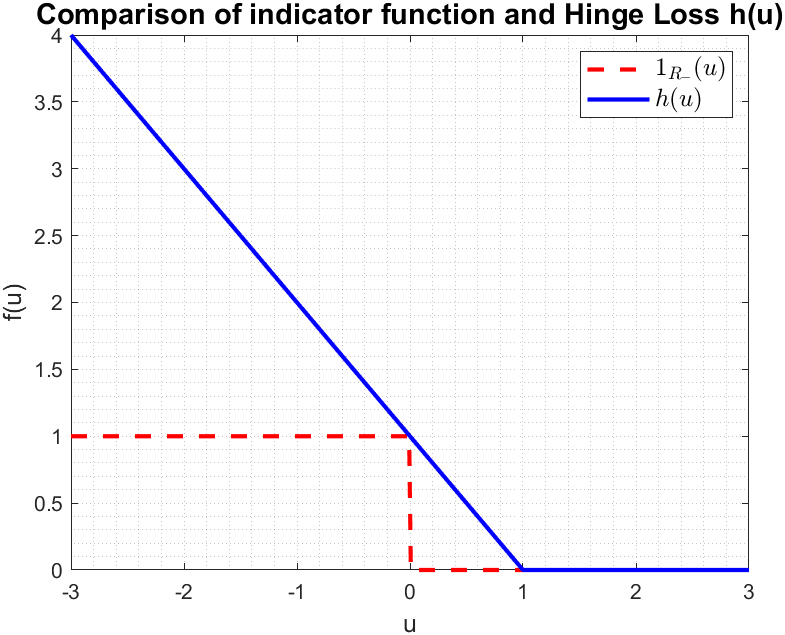
\includegraphics[width=1\linewidth]{Task_2.png}
    \caption{Comparison of the indicator function $\mathbf{1}_{\mathbb{R}_-}(u)$ (red dashed) and the hinge loss function $h(u)$ (blue solid).}
    \label{task_2}
\end{figure}
\vspace{0.3cm}
\textbf{Note: A code that allows to obtain the previous plot is present in the folder documentation.}

\vspace{0.5cm}
{\large\textbf{Discussion of the Graph:}}
\vspace{0.3cm}

As observed in the plot(fig 3.2):
\begin{itemize}
    \item The red dashed line represents the indicator function $\mathbf{1}_{\mathbb{R}_-}(u)$, which takes the value $1$ for $u < 0$ and $0$ for $u \geq 0$.
    \item The blue solid line represents the hinge loss function $h(u) = \max(0, 1 - u)$, which decreases linearly for $u \leq 1$ and is equal to zero for $u \geq 1$.
\end{itemize}

Clearly, the hinge loss function $h(u)$ is always greater than or equal to the indicator function $\mathbf{1}_{\mathbb{R}_-}(u)$, thus confirming the inequality $\mathbf{1}_{\mathbb{R}_-}(u) \leq h(u)$ holds true for all $u \in \mathbb{R}$.

\subsection{Convexity of the Hinge Loss Function}

Finally, we show that $h(u)$ is a convex function. The hinge loss function is piecewise linear, consisting of two linear segments: one with a negative slope for $u < 1$ and another constant at $0$ for $u \geq 1$. Since linear functions are convex, and the pointwise maximum of convex functions is also convex, it follows that $h(u)$ is convex. (ex. $h(u)$ is obviously convex. In fact, for $u \geq 1$, $h(u) = 0$, which is a constant and therefore convex. For $u < 1$, $h(u) = 1 - u$, which is linear and thus convex)


\newpage
% Continue with next tasks...


\newpage

% New page style after the table of contents
\pagestyle{aftertoc}

\section{Task 3: Convexity of the Function $g_D(w_0, w)$}

We are tasked with showing that the function:
\begin{equation}
    g_D(w_0, w) = \frac{1}{N} \sum_{n=1}^{N} h\left(y_n\left(w_0 + x_n^T w\right) \right)
    \label{function_gD}
\end{equation}
is convex for any values of \( N \) and \( D \).

\subsection{Analytical Proof}

Let us begin by decomposing the \eqref{function_gD} function and considering the following properties:

\begin{itemize}
 \item \textbf{Convexity of \( h(u) \):}  
    The function \( h(u) = (1 - u)_+ \), is convex because it is piecewise linear. This has already been demonstrated both analytically and graphically in Task 2 (see Task 2 for reference). The hinge loss function, which \( h(u) \) represents, is well-known to be convex
    
    \item \textbf{Affine Transformation of Variables:}  
    Define \( u_n = y_n(w_0 + x_n^T w) \). Since \( u_n \) is a linear function of \( w_0 \) and \( w \), it is an affine transformation. The composition of a convex function with an affine transformation preserves convexity.
    
    We start with the function:
\begin{equation}
    g_D = \frac{1}{N} \sum_{n=1}^{N} h(u_n)
\end{equation}


where:
\begin{equation}
u_n = y_n(w_0 + x_n^T w) = y_n \left( \begin{bmatrix} x_n^T & 1 \end{bmatrix} \begin{bmatrix} w \\ w_0 \end{bmatrix} \right) =  y_n \cdot \tilde{x}_n^T \cdot \tilde{w} .
\end{equation}

where \( \tilde{x}_n \) and \( \tilde{w} \) are the extended vectors, and it reppresents the linear change of variable u.
But, in general just let focus on  \( h(y_n(w_0 + x_n^T w)) \), since the summation requires another property specification.
The function \( g_D \) is convex in \( \tilde{w} \) because \( h(u) \) is convex and \( u \) represents the result of a linear transformation of the extended variables \( \tilde{x}_n \) and \( \tilde{w} \). 

where \( (w_0 + x_n^T w) \) is an affine function of \( (w_0, w) \), being a linear combination of \( w_0 \) and \( w \).

It is important to notice that aside from the affine function $w_0 + x_n^T w$, $u_n$ also contains a multiplication of the function by the scalar $y_n$. This could also be represented as
\begin{equation} \label{eq:un_definition}
u_n = \begin{cases}
w_0 + x_n^T w & \text{if } y_n = 1, \\
-w_0 + x_n^T (-w) & \text{if } y_n = -1.
\end{cases}
\end{equation}

which does not influence the affinity of the function.

Since \( h(u) \) is convex and \( u_n \) is the result of an affine transformation, we conclude that \( h(y_n(w_0 + x_n^T w)) \) is convex for each \( n \). (Theorem 7.17 states the preservation of convexity under linear change of variables, as detailed in Chapter 7.4 of Amir Beck's book.
Example 7.3 illustrates the convexity of affine functions, and can be found in Chapter 7.1 )

\vspace{0.3cm}
\textbf{Note: All the theorems and examples cited are present in the Amir Beck's book}


    
    \item \textbf{Summation of Convex Functions:}  
    The sum of convex functions remains convex. Since each term in the summation is convex, the entire function \( g_D(w_0, w) \), which is an average of convex functions, remains convex.
Let \( f_1, f_2, \ldots, f_p \) be convex functions defined over a convex set \( C \subseteq \mathbb{R}^n \). Then, the sum function 

\begin{equation}
f = f_1 + f_2 + \ldots + f_p
\end{equation}

is also convex over \( C \). (This property holds true as stated in Theorem 7.16, Chapter 7, Section 7.4, titled "Operations Preserving Convexity").

\item \textbf{Averaging convex functions}:  
Finally, multiplying by \( \frac{1}{N} \), which is a positive scalar, preserves convexity. Thus, the average of convex functions is still convex.

\end{itemize}


Thus, we have shown that $g_D(w_0, w)$ is convex.

\section{Task 4: Convexity of the Second Function $g(w_0, w)$}
We are tasked to prove that the function:
\begin{equation}
g(w_0, w) = \underbrace{\frac{1}{N} \sum_{n=1}^{N} h \left(y_n\left(w_0 + x_n^T w\right)\right)}_{g_D(w_0, w)} + \underbrace{\rho \|w\|_2^2}_{r(w_0, w)}
\label{function_g}
\end{equation}

is convex for any values of $N$ and $D$

\subsection{Analytical Proof}

Beginning with mentally separating the equation \eqref{function_g}, into the sum of the previously proven convex function ($g_D(w_0, w)$), and the rest of the equation ($\rho \|w\|_2^2$); consider the following:

\begin{itemize}
    \item \textbf{Convexity of $g_D(w_0,w)$:} The function \(g_D(w_0, w) = \frac{1}{N} \sum_{n=1}^{N} h(y_n(w_0 + x_n^T w)))\) can be proven that it is in fact convex, when giving use of the theorems stated in Amir Beck's book:
    \begin{itemize}
        \item \textbf{Theorem 7.16 (b)} (preservation of convexity under summation and multiplication by non-negative scalars): for the summation of multiple convex functions, represented by the summatory $\sum_{n=1}^{N}$.
        \item \textbf{Theorem 7.17} (preservation of convexity under linear change of variables): for the composition of a convex function over an affine function.
    \end{itemize}

    In order to conclude if $g(w_0,w)$ is itself convex (following the \textbf{Theorem 7.16 (b)}), we are left to validate if $\rho \|w\|_2^2$ is a convex function.

    Let us consider a bottom-up approach:
    \begin{itemize}
        \item Starting from the basics, it is easily deducible that $\|w\|_2$ will always represent non-negative value.
        \item Applying the square function, a known convex function, to $\|w\|_2$ will always end up in the positive side of the parabola. This familiar situation has been represented in class as $(\cdot)_+^2$. Thus, secured by the \textbf{Theorem 7.22}, we can state that the composition $\|w\|_2^2$ represent a non-decreasing convex function.
        \item Following the \textbf{Theorem 7.16 (a)} we can conclude that the multiplication of the convex function $\|w\|_2^2$ by the non-negative scalar $\rho$, the convexity of the outcome is not affected.
    \end{itemize}

    By following the \textbf{Theorem 7.16 (b)} once another time, we can say that the summation of the convex function \(g_D(w_0, w) = \frac{1}{N} \sum_{n=1}^{N} h(y_n(w_0 + x_n^T w)))\) by the convex function $\rho \|w\|_2^2$ ends up also as convex function.
\end{itemize}

\section{Task 5: Strong Convexity}
For this task, we should investigate the function in \eqref{function_g} to see whether the function is strongly convex or not.
\vspace{0.3cm}

\subsection{Analytical Proof}

\textbf{Strong Convexity (S-CVX):}

In general a function \( f : \mathbb{R}^n \to \mathbb{R} \) is said to be \textit{strongly convex} if there exists a constant \( m > 0 \) such that for all \( x, y \in \mathbb{R}^n \) and \( 0 \leq \alpha \leq 1 \), the following inequality holds:
\begin{equation}
f\left((1 - \alpha)x + \alpha y\right) \leq (1 - \alpha) f(x) + \alpha f(y) - m \frac{\alpha(1 - \alpha)}{2} \|x - y\|^2
\end{equation}

In our case, we need to analyze the function f to see if it is convex or not to determine if the function g is strongly convex:

\begin{equation}
f(w, w_0) = g(w, w_0) - \frac{\beta}{2} \| w \|^2 - \frac{m}{2} w_0^2
\end{equation}

The convexity analysis will be carried out below using two different approaches.

\begin{itemize}
    \item When restricting to $w = 0$ and leaving $w_0$ as a free variable, the regular expression of $f(w, w_0)$:
    \begin{equation}
    f(w, w_0) = \frac{1}{N} \sum_{n=1}^{N} h\left(y_n\left(w_0 + \mathbf{x}_n^T w\right)\right) + \rho \|w\|_2^2 - \frac{\beta}{2} \|w\|_2^2 - \frac{m}{2}w_0^2,
    \label{function_f}
    \end{equation}
    
    which reduced to
    \begin{equation}
    f(w_0) = \frac{1}{N} \sum_{n=1}^{N} h\left(y_n w_0\right) - \frac{m}{2}w_0^2,
    \end{equation}

    takes the values:
    
    \begin{align}
        f(0) &= 0, \\
        \lim_{w_0 \to +\infty} f(w_0) = \lim_{w_0 \to -\infty} f(w_0) &= -\infty
    \end{align}

    The limit value analysis show that the function \eqref{function_f} is not convex, and subsequently the original equation at \eqref{function_g} is not strongly convex. The function f for setting $w$ equal to 0 is also shown in Fig. \ref{disprove_scvx}, where you can clearly see that it is not convex.
    \begin{figure}[h!]
    \centering
        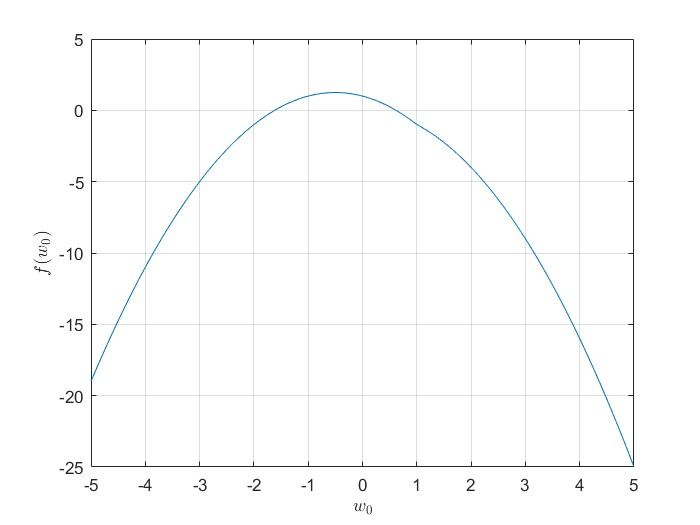
\includegraphics[width=0.8\textwidth]{task_5.jpg}
        \caption{Plot of the function $g$ for setting $\omega = \mathbf{0}$ and $\omega_0$ variable.}
        \label{disprove_scvx}
\end{figure}
    
    \item When $w$ take values such that: $h(y_n(w_0+x_n^Tw)) > 0$
    
\textit{That is} \[
y_n \tilde{x}^T \tilde{\omega} > 0
\]

\textbf{Rewriting the function} \( f(\omega, \omega_0) \):
\begin{equation}
f(\omega, \omega_0) = \frac{1}{N} \sum_{n=1}^{N} y_n (\omega_0 + x_n^T \omega) + \frac{\rho}{2} \|\omega\|_2^2 -\frac{m}{2}\|\omega\|_2^2 - \frac{m}{2} \omega_0^2
\end{equation}

\textbf{Calculating the gradient} \( \nabla f(\omega, \omega_0) \):
\begin{equation}
\nabla f(\omega, \omega_0) = 
\begin{bmatrix}
\frac{1}{N}{\sum_{n=1}^{N} y_n x_n + \rho \omega - m \omega} \\[5pt]
\frac{1}{N} \sum_{n=1}^{N} y_n - m \omega_0
\end{bmatrix}
\end{equation}


\textbf{Computing the Hessian matrix} \( \nabla^2 f(\omega, \omega_0) \):
\begin{equation}
\begin{pmatrix}
\rho & 0 & \cdots & 0 & 0 \\
0 & \rho & \cdots & 0 & 0 \\
\vdots & \vdots & \ddots & \vdots & \vdots \\
0 & 0 & \cdots & \rho & 0 \\
0 & 0 & \cdots & 0 & 0
\end{pmatrix}
\end{equation}

\textit{Observation:} The Hessian matrix is not positive definite.

\textbf{Conclusion on convexity:}
\begin{equation}
\nabla^2 f(\omega, \omega_0) \not\succeq 0 \quad \Rightarrow \quad \text{the function is not convex!}
\end{equation}

\textit{Conclusion:} This proofs the intuition from plot \label{} that the function in \eqref{function_g} is not strongly convex.


    
\end{itemize}


\section{Task 6: Numerical Solution Using CVX}

In this task, we aim to solve  the following problem using the CVX toolbox.
\begin{equation}
\min_{w_0, w} \quad \frac{1}{N} \sum_{n=1}^{N} h\left(y_n\left(w_0 + \mathbf{x}_n^T w\right)\right) + \rho \|w\|_2^2,
\end{equation}
\[
\underbrace{\left( \frac{1}{N} \sum_{n=1}^{N} h\left(y_n \left(w_0 + \mathbf{x}_n^T w\right)\right) \right)}_{g_D(w_0, w)} + \underbrace{\rho \|w\|_2^2}_{r(w_0, w)}
\]

 Using the parameters \((w_0, w)\) obtained from the solution of the previous problem , we evaluate the performance of the classifier \(C_{w_0, w}(x)\), defined as:

\[
C_{w_0, w}(x) = \text{sign}(w_0 + x^T w),
\]

In the appendix, we present the code used to solve this problem, along with comments for clarity.
After running the code, it is possible to obtain the following results for the case $\rho = 0.1$ and $\rho = 0.5$ respectably: \\


%\vspace{0.5cm}
%\noindent

%\begin{minipage}[t]{0.48\textwidth}
%    \begin{description}
%        \item[Status:]{Solved}
%        \item[Optimal value (cvx\_optval):]{+0.0342602}
%        \item[Training error rate:]{0.00\%}
%        \item[Test error rate:]{0.12\%}
%    \end{description}
%\end{minipage}
%\begin{minipage}[t]{0.48\textwidth}
%    \begin{description}
%        \item[Status:]{Solved}
%        \item[Optimal value (cvx\_optval):]{+0.103117}
%        \item[Training error rate:]{0.25\%}
%        \item[Test error rate:]{0.25\%}
%    \end{description}
%\end{minipage}

%\vspace{0.5cm}
%\noindent
\begin{minipage}[t]{0.48\textwidth}
    % Table for rho = 0.1
    \centering
    \rowcolors{2}{blue!10}{blue!10}
    \begin{tabular}{|p{6cm}|}
    \hline
    \rowcolor{blue!30}
    \textbf{Results with $\rho = 0.1$} \\
    \hline
    \textbf{Status:} Solved \\
    \textbf{Optimal value (cvx\_optval):} +0.0342602 \\
    \textbf{Training error rate:} 0.00\% \\
    \textbf{Test error rate:} 0.12\% \\
    \hline
    \end{tabular}
\end{minipage}%
%\hfill
\begin{minipage}[t]{0.48\textwidth}
    % Table for rho = 0.5
    \centering
    \rowcolors{2}{blue!10}{blue!10}
    \begin{tabular}{|p{6cm}|}
    \hline
    \rowcolor{blue!30}
    \textbf{Results with $\rho = 0.5$} \\
    \hline
    \textbf{Status:} Solved \\
    \textbf{Optimal value (cvx\_optval):} +0.103117 \\
    \textbf{Training error rate:} 0.25\% \\
    \textbf{Test error rate:} 0.25\% \\
    \hline
    \end{tabular}
\end{minipage}

\vspace{0.5cm}

Therefore, we can conclude that our analysis for task 6 is complete.
\vspace{0.1cm}

\textit{Note: You can achieve the same result using a for loop. Of course, using "tic-toc" command, you can see that this is not an optimal choice, since it requires more calculation time.}




\section{Task 7: Designing the worst attack to a feature vector}
In this task you will be dealing with a problem of worst attack to a feature vector. Given the feature vector $x$ as: 
\begin{equation}
    x = x_d =\begin{bmatrix} x_1 \\ x_2 \\x_3 \end{bmatrix} \quad  d = 1, \cdots, 3
\end{equation}
category $y$ of a feature vector $x$, classifier parameters $(\omega_0,\omega)$ and known that attacker can change every components of $x$ in:
\begin{equation}
    \tilde{x} = \tilde{x}_d =\begin{bmatrix} \tilde{x_1} \\ \tilde{x2} \\ \tilde{x_3} \end{bmatrix} \quad  d = 1, \cdots, 3
\end{equation}
\begin{equation}
    \tilde{x} =[x_d - P; x_d + P] \quad \text{in this case }\quad P = 0,5 \nonumber
\end{equation}
the goal of the attacker is solve:
\begin{flalign}
    & \min_{\tilde{x}} \quad y(w_0 + {\tilde{x}}^T w) \label{eq:min_function}\\
    & \text{subject to} \quad |\tilde{x}_d - x_d| \leq P, \quad \text{for }\quad  1 \leq d \leq D \nonumber
\end{flalign}
where P is the maximal deviation the attacker can introduce\\

The aims of this task were:\\
\textbf{a)} show that $\tilde{x} = x - P \operatorname{sgn}(yw)$ solves the cost function above \eqref{eq:min_function}\\
\textbf{b)} show that, for such $\tilde{x}$, \eqref{eq:min_function} evaluates to $y(w_0 + {x}^T w) - P \|{y \omega}\|_1$

\subsection{Analytical Proof}
\textbf{a)} First of all, we can note that the function $y(w_0 + {\tilde{x}}^T w)$ can be written as:
\begin{align}
    y(w_0 + {\tilde{x}}^T w) = y w_0 + y {\tilde{x}}^T w = y w_0 + (y {\tilde{x}_1}^T w + \cdots + y {\tilde{x}_d}^T w)
\end{align}
Attacker goal is to minimize $y(w_0 + {\tilde{x}}^T w)$; we must therefore modify $\tilde{x}$ as to try to force this quantity to be negative. The optimal strategy to minimize \eqref{eq:min_function} is to modify each component $\tilde{x}$ in such a way that the value of ${x}^T w$ is reduced as much as possible i.e. $\tilde{x}$ need to be chosen:
\begin{itemize}[label=-]
     \item as large as possible if $\operatorname{sgn}(yw) < 0$.
     \item as small as possible if $\operatorname{sgn}(yw) > 0$.
\end{itemize}

$\tilde{x}$ is in the interval $[x_d - P; x_d + P]$ and should be set to the marginal values of the interval depending on the sign of of $y \omega$. The value $\tilde{x}^T w$ is minimized when $x$ takes the value farthest in the opposite direction of $\omega_0$ i.e. when:
\begin{equation}
    \tilde{x} = x - P \operatorname{sgn}(yw) = \tilde{x} 
    \begin{bmatrix}
        x_1 - P \operatorname{sgn}(yw_1) \\[5pt]
        \cdots \\[5pt]
        x_d - P \operatorname{sgn}(yw_d)
    \end{bmatrix}
\end{equation}

\textbf{b)} The cost function we have to minimize is \eqref{eq:min_function}. Knowing that:\begin{equation}
\tilde{x} = x - P \operatorname{sgn}(yw) = \tilde{x} 
\end{equation} 
we can we can rewrite \eqref{eq:min_function} as follows;
\begin{flalign}
    & y(w_0 + {\tilde{x}}^T w) = \label{eq:x-Psgn(yn)}\\
    & y(w_0 + ( x - P \operatorname{sgn}(yw))^T \omega) = \nonumber \\
    & y(w_0 + {x}^T w) - y P \operatorname{sgn}(yw)^T \omega = \nonumber \\
    & y(w_0 + {x}^T w) - P (\operatorname{sgn}(yw_1) \cdot yw_1 + \cdots + \operatorname{sgn}(yw_d)  \nonumber
 \cdot yw_d)
\end{flalign}
now knowing the \textbf{sign property} according to which:
\begin{equation}
    \operatorname{sgn}(yw) \cdot yw = |yw| 
\end{equation}
and \textbf{$\emph{l}_1 -$norm property}:
\begin{equation}
    |yw_1| + \cdots + |yw_d| = \|yw\|_1 
\end{equation}
\eqref{eq:x-Psgn(yn)} thus becomes:
\begin{flalign}
    & y(w_0 + {x}^T w) - P \|yw\|_1
\end{flalign}


\section{Task 8}
In this task, the data set was attacked by modifying the feature vector accordingly: 
\begin{equation}
    \tilde{x} = x - P \, \mathrm{sgn}(yw)
\end{equation}
After the attack on the data set, you can see a strong increase in the error rate of the classifier ($\rho=0.1$) : 
\begin{description}
\item[attacked test dataset:]{$43.56\%$}
\end{description}

\section{Task 9}
This task is about designing a classifier that is robust against attacks on the dataset. Therefore, the classifier needs to be retrained based on a different cost function that takes into account that the feature vector is manipulated. 

For a hyperparameter configuration of $\rho=0.1$, the robust classifier achieves the following error-rate: 
\begin{description}
\item[train dataset:]{0.75\%}
\item[test dataset:]{0.44\%}
\item[attacked test dataset:]{$2.19\%$}
\end{description}

These results indicate that the robust classifier is highly effective. The low error rates on both the training and test datasets, demonstrate good performance.Although the error rate increases to {$2.19\%$} on the attacked test dataset, it’s still relatively low, suggesting that the classifier maintains resilience against adversarial manipulations. The result is really incredible if we compare it with the result obtained in task 8.


\section{Task 10}
In this task the goal is to fit a mixture of linear models to a nonlinear function. The mixture of linear models 
\begin{equation}
    \hat{y}(x) = \sum_{k=1}^{K} w_k(x) \hat{y}_k(x)
\end{equation}
is a composition of linear functions 
\begin{equation}
    \hat{y}_k(x) = s_k x + r_k
\end{equation}
, where each linear function is weighted by a weighting parameter:
\begin{equation}
    w_k(x) = \frac{e^{u_k x + v_k}}{e^{u_1 x + v_1} + \cdots + e^{u_K x + v_K}} .
\end{equation}
The mixture of linear mixture models is parametrized by the parameter vector
\begin{equation}
    \theta = [s_1, r_1, \dots, s_K, r_K, u_1, v_1, \dots, u_{K-1}, v_{K-1}]^T
\end{equation}
, which should be determine such that the objective function $f(\theta)$ is minimized:
\begin{equation}
    \min_{} f(\theta) =  
\sum_{n=1}^{N} {\underbrace{\left( \hat{y}_{n}(\theta) - y_n \right)}_{=:f_n(\theta)}}^2 .
\end{equation}
The loss function can be minimized using the Levenberg-Marquardt (LM) algorithm. To apply the algorithm, the gradient of the functions $f(\theta)$ and $f_n(\theta)$ need to be determine. The gradient of f can be simply calculated by applying the chain rule: 
\begin{equation}
    \nabla f(\theta) =  2 \sum_{n=1}^{N} f_n(s,r,u,v) \nabla f_n (s,r,u,v). 
\end{equation}
To calculate the gradient of $f_n$, this can be done by looking at the partial derivatives 
\begin{flalign}
   & \frac{\partial{f_n}}{\partial{s_i}} = w_i  x_n , \\
   & \frac{\partial{f_n}}{\partial{r_i}} = w_i , \\
   & \frac{\partial{f_n}}{\partial{u_i}} = \left( \sum_{k=1}^{K} -w_k w_i \hat{y}_k + w_i \hat{y}_i \right) x_n , \\
   & \frac{\partial{f_n}}{\partial{v_i}} = \sum_{k=1}^{K} -w_k w_i \hat{y}_k + w_i \hat{y}_i    .
\end{flalign}
, where $i = 1,\ldots,K$. 
The LM-algorithm was implemented in Matlab (see \ref{}) and the algorithm stops when the gradient of f drops under $\epsilon = 10^{-4}$ or a maximum number of 5000 iterations is reached. In our case, the algorithm stopped after 78 iterations, where the following values for our optimization variables are obtained: 
\[
u = \begin{bmatrix}
   -13.0771 \\ -80.1045 \\ 88.2025
  \end{bmatrix}, \quad 
  v = \begin{bmatrix}
   -2.3460 \\ -415.5622 \\ -184.8455
\end{bmatrix}, \quad 
s = \begin{bmatrix}
  -1.2015 \\ 3.2655 \\ -3.9997 \\ 12.1257
\end{bmatrix}, \quad 
r = \begin{bmatrix}
  -0.0769 \\ 23.0588 \\ 19.8766 \\ -2.6533
\end{bmatrix} .
\]
This results in the weighting parameters shown in the fig. \ref{task_10_weights}, which clearly shows the sections in which the non-linear function is approximated by linear functions. 
\begin{figure}[htbp]
    \centering
        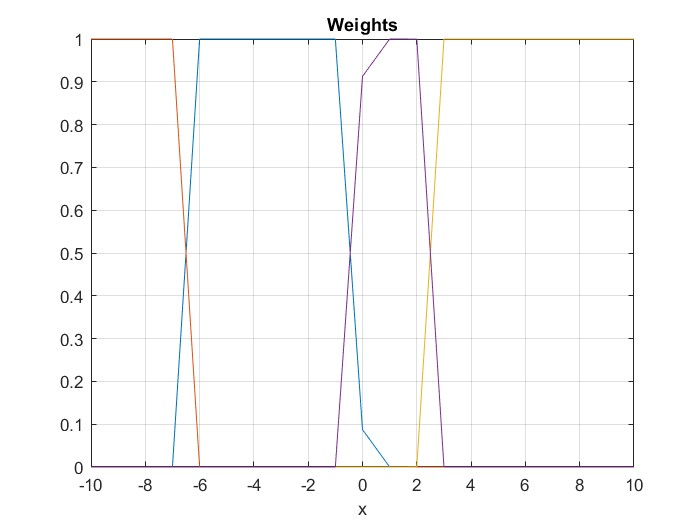
\includegraphics[width=0.8\textwidth]{task_10_weights.jpg}
        \caption{The $K=4$ weight functions, each weight is plotted in a different color.}
        \label{task_10_weights}
\end{figure}
The transient behavior of the loss function and the gradient of the the loss function are given in fig. \ref{task_10_iterations}. 
\begin{figure}[htbp]
  \centering
  \begin{subfigure}[b]{0.49\textwidth}
    \centering
    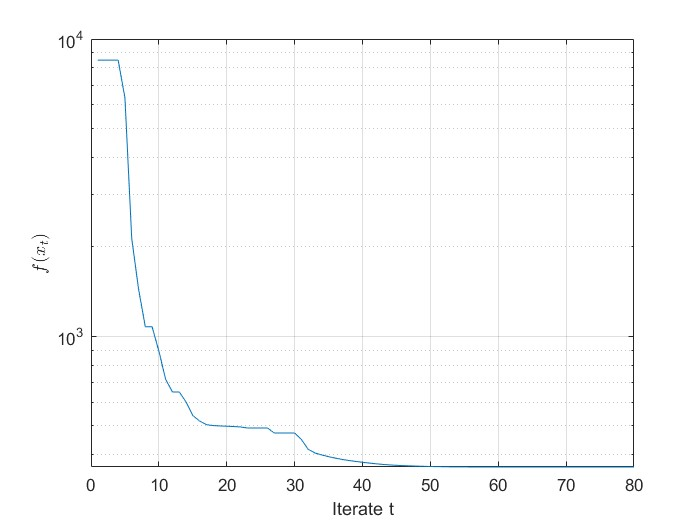
\includegraphics[width=\textwidth]{task_10_loss.jpg}
    \caption{}
    \label{task_10_loss}
  \end{subfigure}
  \hfill
  \begin{subfigure}[b]{0.49\textwidth}
    \centering
    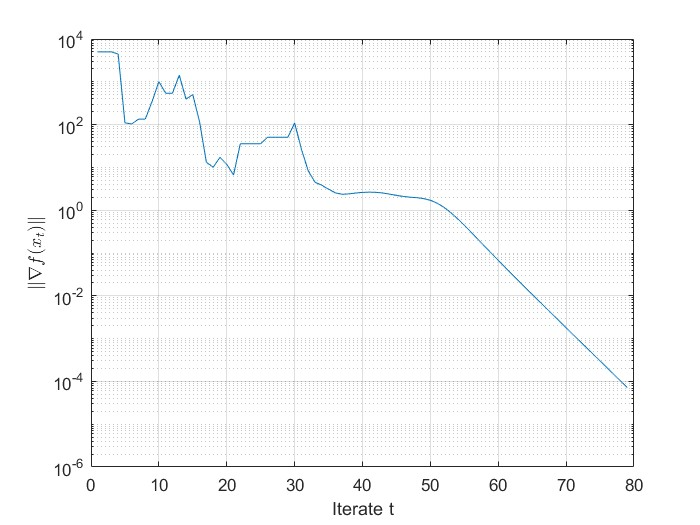
\includegraphics[width=\textwidth]{task_10_gradient.jpg}
    \caption{}
    \label{task_10_gradient}
  \end{subfigure}
  \caption{The value (a) and the norm of the gradient (b) of the objective function of across the LM iterates.}
  \label{task_10_iterations}
\end{figure}
Finally, the result of the approximation of the nonlinear function $y$ by the mixture of the linear function $\hat{y}$ is shown in fig. \ref{task_10_mixture_LM}. It can be clearly seen that the approximation corresponds well to the underlying function.
\begin{figure}[htbp]
    \centering
        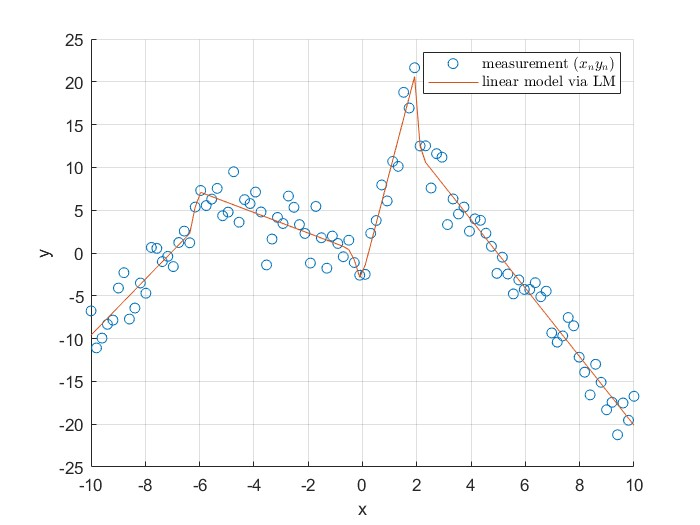
\includegraphics[width=0.8\textwidth]{task_10_mixture_LM.jpg}
        \caption{Approximation of the respective function using a mixture of linear models.}
        \label{task_10_mixture_LM}
\end{figure}


\chapter{Appendix: Matlab Code Task}

\subsection{Task 6 Code}
Below, we present the code used to solve this problem, along with comments for clarity.

\begin{lstlisting}[language=Matlab, style=Matlab-editor, frame=single, numbers=left]
%% setup the data
% load data from workspace
load("dataset/classifier_dataset.mat");

% define variables
Ntrain = size(traindataset, 1); D = 784;
Ntest = size(testdataset, 1);
n = D + 1;  % Corrected to D + 1
ytrain = trainlabels;
Xtrain = [traindataset ones(Ntrain, 1)];  % Adding bias term
ytest = testlabels;
Xtest = [testdataset ones(Ntest, 1)];  % Adding bias term

% configuration of the hyperparameters
rho = 0.1;

%% solving the convex optimization problem
cvx_begin quiet
    variable w(n)  
    minimize(1/Ntrain * sum(max(0, 1 - ytrain .* (Xtrain * w))) + rho * square_pos(norm(w(1:D))));  
cvx_end

%% evaluation of the performance
% testing on trainset
eps = ytrain .* (Xtrain * w);
eps(eps>0) = 0; 
eps(eps<0) = 1; 
errtrain = 1/Ntrain * sum(eps);
% testing on testset
eps = ytest .* (Xtest * w);
eps(eps>0) = 0;
eps(eps<0) = 1; 
errtest = 1/Ntest * sum(eps);

% return error 
fprintf('Train error [%%]: %.2f\n', errtrain * 100);
fprintf('Test error [%%]: %.2f\n', errtest * 100);

\end{lstlisting}



\subsection{Task 8 Code}
Below, the code for resolution of task 8:
\begin{lstlisting}[language=Matlab, style=Matlab-editor, frame=single, numbers=left]
%% setup the data
% load data from workspace
load("dataset/classifier_dataset.mat");

% configuration of the hyperparameters
rho = 0.1;
P = 0.18;

% load w
load(['w_' num2str(rho)]);

% define variables
Ntrain = size(traindataset, 1); D = 784;
Ntest = size(testdataset, 1);
n = D + 1;  % Corrected to D + 1
ytrain = trainlabels;
ytest = testlabels;
Xtrain = traindataset; 
Xtest_attack = testdataset;

% attack the dataset
Xtest_attack = Xtest_attack - P*sign(ytest*w(1:D)');

% adding bias term
Xtrain = [Xtrain ones(Ntrain, 1)];
Xtest_attack = [Xtest_attack ones(Ntest, 1)];

%% evaluation of the performance
% testing on trainset
eps = ytrain .* (Xtrain * w);
eps(eps>0) = 0; 
eps(eps<0) = 1; 
errtrain = 1/Ntrain * sum(eps);
% testing on testset
eps = ytest .* (Xtest_attack * w);
eps(eps>0) = 0;
eps(eps<0) = 1; 
errtest = 1/Ntest * sum(eps);

% return error 
fprintf('Train error [%%]: %.2f\n', errtrain * 100);
fprintf('Test error [%%]: %.2f\n', errtest * 100);
\end{lstlisting}


\subsection{Task 9 Code}
The code for Task 9 for training the model and performance evaluation is given below.
\begin{lstlisting}[language=Matlab, style=Matlab-editor, frame=single, numbers=left]
%% setup the data
% load data from workspace
load("dataset/classifier_dataset.mat");

% configuration of the hyperparameters
rho = 0.1;
P = 0.18;

% define variables
Ntrain = size(traindataset, 1); 
D = 784;
Ntest = size(testdataset, 1);
ytrain = trainlabels;
ytest = testlabels;
Xtrain = traindataset; 
Xtest = testdataset;

% Adding bias term 
Xtrain = [Xtrain ones(Ntrain, 1)];
Xtest = [Xtest ones(Ntest, 1)];

%% solving the convex optimization problem
cvx_begin quiet
    variable w(D+1)  
     minimize(1/Ntrain * sum(max(0, 1 - (ytrain .* (Xtrain * w) - P * abs(ytrain)*abs(w(1:D)')*ones(D,1)))) + rho * square_pos(norm(w(1:D))));  
cvx_end

%% Attacking
%attack the dataset
Xtest_attack = testdataset;
Xtest_attack = Xtest_attack - P*sign(ytest*w(1:D)');
Xtest_attack = [Xtest_attack ones(Ntest, 1)];

%% evaluation of the performance
% testing on trainset
eps = ytrain .* (Xtrain * w);
eps(eps>0) = 0; 
eps(eps<0) = 1; 
errtrain = 1/Ntrain * sum(eps);
% testing on testset
eps = ytest .* (Xtest * w);
eps(eps>0) = 0;
eps(eps<0) = 1; 
errtest = 1/Ntest * sum(eps);
% testing on attacked data
eps = ytest .* (Xtest_attack * w);
eps(eps>0) = 0;
eps(eps<0) = 1; 
errtest_attack = 1/Ntest * sum(eps);

% return error 
fprintf('Train error [%%]: %.2f\n', errtrain * 100);
fprintf('Test error [%%]: %.2f\n', errtest * 100);
fprintf('Test error attack [%%]: %.2f\n', errtest_attack * 100);
\end{lstlisting}


\subsection{Task 10 Code}
\begin{lstlisting}[language=Matlab, style=Matlab-editor, frame=single, numbers=left]
%% setup the data
% load data from workspace
load("dataset/lm_dataset_task.mat");

% initilize parameters
K = size(s,1); 
N = size(y,1);
n = 14;
lambda = 1; 
eps = 1e-4;
iter = 5000; %5000
cnt = 0;
 
% Calculate initial values
f = 0;
gradf = 0;
for j = 1:N 
    [fp, gradfp] = func_eval(x(j),y(j), r, s, v, u);
    f = f + fp^2;
    gradf = gradf + 2*fp * gradfp;       
end

% log data
history.f = f;
history.lambda = lambda;
history.gradf = norm(gradf);
history.f(end+1) = f;

%% LM algorithm 
while norm(gradf) > eps & cnt < iter
    % constructing Least-Square problem
    A = zeros(N+n,n);
    b = zeros(N+n,1);
    for i = 1:N
        [fp, gradfp] = func_eval(x(i),y(i), r, s, v, u);
        A(i,:) = gradfp;
        b(i) = gradfp'* [r;  s;  v;  u] - fp ;
    end
    A(N+1:end,:) = lambda^0.5 * eye(n); 
    b(N+1:end) = lambda^0.5 * [r;  s;  v;  u]; 
    
    % solving Least-Square problem
    theta = A\b;
    x_r = theta(1:4); x_s = theta(5:8); x_v = theta(9:11); x_u = theta(12:14);   

    % evaluation function at new value
    fnew = 0;
    gradfnew = 0;
    for j = 1:N
            %fnew = fnew + func(x(j),y(j), x_r, x_s, x_v, x_u)^2;  
            [fp, gradfp] = func_eval(x(j),y(j), x_r, x_s, x_v, x_u);
            fnew = fnew + fp^2;
            gradfnew = gradfnew + 2*fp * gradfp; 
    end

    % check update parameters
    if fnew < f 
        % update function value 
        f = fnew;
        % update parameters
        r = x_r; s = x_s; v = x_v; u = x_u;        
        % update new gradient
        gradf = gradfnew;      
        % decrease step size        
        lambda = 0.7 * lambda;        
    else
        lambda = 2 * lambda;
    end 
     % log data 
     history.f(end+1) = f; 
     history.gradf(end+1) = norm(gradf);
     history.lambda(end+1) = lambda;
     cnt = cnt + 1;
     disp(['iteration: ', num2str(cnt), ', loss: ', num2str(history.f(end)), ', norm gradient: ', num2str(history.gradf(end))]);
end
% log final parameters
history.r = r;
history.s = s;
history.v = v;
history.u = u;

function [f, gradf] = func_eval(x, y, r, s, v, u)
    u = [u ; 0];
    v = [v; 0];    

    % Calculate alpha
    alpha = u * x + v;
    alpha_bar = max(alpha);

    % Calculate w_k(x_n) 
    wx_numer = exp(alpha - alpha_bar);     
    wx_denom = sum(wx_numer);  
    w_k = wx_numer / wx_denom;

    % Calculate y_hat_k
    y_hat_k = s * x + r;

     % Calculate the overall y_hat(x_n)
     y_hat = sum(w_k .* y_hat_k);
        
     % Compute the error term (y_hat - y_n)
     f = y_hat - y;   
    
 	% Comupte the gradients
    grad_r = w_k;
    grad_s = grad_r * x;
    grad_v = sum(-w_k .* y_hat_k * w_k', 1)' + w_k .* y_hat_k;
    grad_u = grad_v * x;
    
    grad_u(end) = [];
    grad_v(end) = [];
    gradf = [grad_r; grad_s; grad_v; grad_u];
    
end

\end{lstlisting}



% Bibliografia
\newpage
\addcontentsline{toc}{chapter}{References}
\section*{References}

\begin{enumerate}
    \item \url{https://github.com/Linux-99/Optimization-and-Algorithms-Group-IST-} (Group’s Github Project page)
    \item “Slides Optimization and Algorithms,” 2024, Team: Joao Xavier, Joao Sequeira, Hugo Pereira
    \item \url{https://cvxr.com/cvx/} (CVX: MATLAB Software for Disciplined Convex Programming) (Needed to solve the tasks)
    \item “Optimization and Algorithms: Proofs of the Theorems in the Slides,” 2024, João Xavier.
    \item “Introduction to NonLinear Optimization,” Amir Beck, (Chapter 7 “Convex Functions”; 7.4 (Operations Preserving Convexity))
\end{enumerate}

\appendix 


\end{document}




The objective function \( g_D \) is defined as follows:
\[
g_D = \frac{1}{N} \sum_{n=1}^{N} h(u_n)
\]
where:
\[
u_n = y_n(w_0 + x_n^T w) = y_n \left( \begin{bmatrix} x_n^T & 1 \end{bmatrix} \begin{bmatrix} w \\ w_0 \end{bmatrix} \right).
\]

